% ----------------------------------------------- 
%  Plantilla LaTeX para el Trabajo Fin de Grado
%         Facultad de Ciencias
%        Universidad de Córdoba
%             Codificación utf8
%------------------------------------------------
%              Abril 2022
%------------------------------------------------
\documentclass[12pt,a4paper]{report}

% Fichero de estilo proporcionado
%%%%%%%%%%%%%%%%%%%%%%%%%%%%%%%%%%%%%%%%%%%%%%%%%%%%
%%
%% Este es el fichero 'estilo_TFG_CienciasUCO_2022.sty'
%%    con el estilo LaTeX para escribir los
%%          TRABAJOS FIN DE GRADO
%%                 de la 
%%          Facultad de Ciencias 
%%         Universidad de Córdoba
%               Abril 2022
%    
%           CODIFICAIÓN utf-8
%%%%%%%%%%%%%%%%%%%%%%%%%%%%%%%%%%%%%%%%%%%%%%%%%%%%%



% Idioma castellano 
\usepackage[utf8]{inputenc}
\usepackage[T1]{fontenc}
\usepackage[spanish,es-tabla]{babel}
%\usepackage{mathpazo} 
%\usepackage{eulervm}


% Tamaño de la página
\usepackage[left=2.5cm,right=2.5cm,top=2cm,bottom=2cm]{geometry}

% Para redefinir algunas cosas del babel en castellano 
\accentedoperators    % Pone acentos a los operadores
\decimalpoint         % Usa el punto como separador decimal
                    

% Paquetes auxiliares  (incluir aquellos que se necesiten)

\usepackage[usenames,dvipsnames]{xcolor} % Para usar colores
\usepackage{tikz}                        % Para dibujar
\usepackage[strict]{changepage}          % Para redefinir márgenes en mitad del documento
\usepackage{csquotes}
\usepackage{amsmath}
\definecolor{customblue}{RGB}{81,167,228}
\definecolor{customgreen}{RGB}{117,167,88}
\usepackage{enumitem} 
\usepackage{comment}
\usepackage{units}


% Para matemáticas
\usepackage{amsmath}
\usepackage{amsfonts}
\usepackage{amssymb}

% Para gráficos
\usepackage{graphicx}
\usepackage{subfigure}
\usepackage{float}
%
\usepackage{appendix}   % Contiene mandatos adicionales para apéndices
\usepackage{titlesec}   % Para redefinir capítulos, secciones,...
\usepackage{longtable}  % Para tablas grandes


% Para las cabeceras y pies (luego se redefine cuando haga falta)
\usepackage{fancyhdr}   % Para las cabeceras
\pagestyle{fancy} 
\fancyhf{}
\renewcommand{\headrulewidth}{0pt}
\renewcommand{\footrulewidth}{0pt}

%% captions
\usepackage{subcaption}
\DeclareCaptionFormat{custom}
{%
    \textbf{#1#2}\textit{\small #3}
}
\captionsetup{format=custom, width=0.9\textwidth, font={small, onehalfspacing}}

%Para el fondo de la portada
\usepackage{eso-pic}
\newcommand\BackgroundPic{%
\put(0,0){%
\parbox[b][\paperheight]{\paperwidth}{%
\vfill
\centering

\includegraphics[width=\paperwidth,height=\paperheight,%
keepaspectratio]{fondo_portada.png}%
\vfill
}}}

% Estilo de capítulo, secciones...

\titlespacing*{\chapter}{0pt}{50pt}{40pt}
\titleformat{\chapter}[display]
  { \sffamily\bfseries\Large\color{blue}}
  {\filleft\MakeUppercase{\chaptertitlename}\ \Huge\sffamily{\arabic{chapter}}\ 
  }  
  {4ex}
  {\titlerule
   \vspace{2ex}%
   \filright}
  [\vspace{2ex}\hrule\vspace{2pt}%
   \titlerule]
   
   \titleformat{\section}[hang]
{\large \scshape\bfseries}
{\color{blue}  \thesection .}
{1ex}{\color{blue}}[\quad]
{}

  \titleformat{\subsection}[runin]
{ \scshape\bfseries}
{\color{blue}  \thesubsection .}
{1ex}{\color{blue}}[\quad]
{}

%%%%%%%%%%%%%%%%%%%%%%%%%%%%%%%%%%%%
% Para los códigos 
\usepackage{listings}

% Para código Matlab
\lstset{language=Matlab,
  keywords={break,case,catch,continue,else,elseif,end,for,function,
      global,if,otherwise,persistent,return,switch,try,while,diary,
      clear,clc,who,whos,help,helpwin,linspace,length,ans,doc,floor,
      ceil,max,min,sum,prod,sort,round,sign,fix,mean,exp,sin,cos,tan,
      input,fprint,load,save,disp,fopen,fclose,inline,function,feval,
      global,return,poly,polyval,roots,solve,fzero, poly2sym,hold,plot,
      polyfit,ppval,spline,interp1,quad,quadl,quadgk,inv,\,lu,cond,spdisgs,
      magic,ode*,ode45,ode23,flops,rref,pinv,chol,zeros,ones,rand,sparse,
      tic,toc,diag,eye,speye,espones,spy,syms,diff,dsolve,simplify,ezplot},
   basicstyle=\small \ttfamily,
   keywordstyle=\color{blue},
   commentstyle=\color{webgreen},
   stringstyle=\color{webtinto},
   numbers=left,
   numberstyle=\tiny\color{gray},
   stepnumber=1,
   numbersep=10pt,
   backgroundcolor=\color{white},
   tabsize=4,
   showspaces=false,
   showstringspaces=false,
%
   frame=LtbR,
     framerule=0.5pt,
     aboveskip=0.5cm,
     framextopmargin=3pt,
     framexbottommargin=3pt,
%     framexleftmargin=1cm,
     framesep=0pt,
     rulesep=.4pt,
     backgroundcolor=\color{gray96},
     rulesepcolor=\color{black}}
     
     
 % Para código ISE
     
\lstdefinelanguage{ISE} {morekeywords={library,use,entity,is,port,in,out,end,
               architecture,of,is,signal,begin,process,then,
               port,downto,if,and,then,else
               },                
sensitive=false,
emph={STD_LOGIC_1164,
STD_LOGIC_ARITH,
STD_LOGIC_UNSIGNED,
IEEE,
ALL,
STD_LOGIC,
STD_LOGIC_VECTOR}, 
emphstyle=\color{magenta},
morecomment=[l]{--},
basicstyle=\small \ttfamily,
   keywordstyle=\color{blue},
   commentstyle=\color{webgreen},
   stringstyle=\color{webtinto},
   numbers=left,
   numberstyle=\tiny\color{gray},
   stepnumber=1,
   numbersep=10pt,
   backgroundcolor=\color{white},
   tabsize=4,
   showspaces=false,
   showstringspaces=false,
%
   frame=LtbR,
     framerule=0.5pt,
     aboveskip=0.5cm,
     framextopmargin=3pt,
     framexbottommargin=3pt,
%     framexleftmargin=1cm,
     framesep=0pt,
     rulesep=.4pt,
     backgroundcolor=\color{gray96},
     rulesepcolor=\color{black}
     }
     
%para generar índice con hipervínculos
\usepackage{hyperref} 



\hypersetup{
    colorlinks,
    citecolor=webgreen,
    filecolor=black,
    linkcolor=webblue,
    urlcolor=webtinto,
}


% Colores definidos
\definecolor{azul}{rgb}{65,105,225}
\definecolor{webgreen}{rgb}{0,.5,0}
\definecolor{webgray}{rgb}{.753,.753,.753}
\definecolor{webblue}{rgb}{0,0,.8}
\definecolor{webtinto}{rgb}{0.73,0.00,0.00}
\definecolor{gray96}{gray}{.96}

% Algunas redefiniciones 
%\renewcommand{\contentsname}{Índice general}
%\renewcommand{\partname}{Parte}
%\renewcommand{\appendixname}{Apéndice}
%\renewcommand{\figurename}{Figura}
%\renewcommand{\listfigurename}{Índice de figuras}
%\renewcommand{\chaptername}{Capítulo}
%\renewcommand{\bibname}{Bibliografía}




%%%% Nuevas definiciones %%%%%%%%%%%%%%%%%%%%%%%%%%%%%%%

% Ejemplos de algunas definiciones 
\def\dint{\displaystyle \int}
\def \gt {\gamma(t)}        %  gamma(t)
\def \st {\tilde{\sigma}}   %  sigma tilde
\def \sg {\sigma_{\gamma}}  %  sigma sub gamma
\def \omt {\omega(t)}       %  omega(t)
\def \bu {\mathbf{u}}       %  u negrilla
\def \R {\mathbb{R}}        %  números reales


%--------------------------------------------------------------------------------------
% CAMBIAR LOS DATOS EN CADA CASO 

\newcommand{\titulacion}{Grado de Física}                  % Grado de Biología
                                                      % Grado de Bioquímica
                                                      % Grado de Ciencias Ambientales
                                                      % Grado de Física
                                                      % Grado de Química
                                                      
\newcommand{\titulo}{Luminescent response study of ionic crystals used in dosimetry} % Título
\newcommand{\codigo}{FS24-008-FSC}      % Código
\newcommand{\tipo}{Trabajo de iniciación a la investigación}             % Trabajo teórico--práctico general
                                          		     % Trabajo de iniciación a la investigación
                                                      % Trabajo en empresa
                                                      % Idea de negocio
                                                      % Propuesta científico--técnica
                                                      % Trabajo docente
                                          
\newcommand{\autor}{Marta de la Rosa Núñez}     % Autor
\newcommand{\fecha}{Fecha de entrega}                 % Fecha de entrega
%--------------------------------------------------------------------------------------
\newcommand{\nomfig}{Figura}                         
\newcommand{\nomfigs}{figuras} 

% Si se quiere que las figuras se denominen ilustraciones comentar las dos órdenes
% anteriores y descomentar las dos que siguen 

%\newcommand{\nomfig}{Ilustración}                         
%\newcommand{\nomfigs}{ilustraciones}   


%--------------------------------------------------------------------------------------

% Empieza el documento
\begin{document}

% No cambiar  %%%%%%%%%%%%%%%%%%%%%%%%%%%%%%%%%%%%%%%%%%%%%%%%%%%%%%%%%%%%
%%%%%%%%%%    NO CAMBIAR   %%%%%%%%%%%%%%%%%%%%%%%%%%%%%
% Inclusión automática de la portada, tribunal e índices
%%%%%%%%%%    NO CAMBIAR   %%%%%%%%%%%%%%%%%%%%%%%%%%%%%%

% PORTADA----------------------------------
\AddToShipoutPicture*{\BackgroundPic}
\begin{titlepage}
\begin{center}
\Large UNIVERSIDAD DE CÓRDOBA\\[0.5 cm]
\large  \textbf{Facultad de Ciencias}\\[1.25 cm]
\large \textbf{\titulacion}\\[1.25 cm]
\Large  Trabajo Fin de Grado\\[2.25 cm]
\Huge   \titulo
\end{center}
\vspace{1.25cm}
\noindent {\large Código del TFG: \textbf{\color{blue}\codigo}}\\[0.3cm]
\noindent {\large Tipo de TFG: \textbf{\color{blue}\tipo}}\\[0.5cm]
{\color{blue}\hrule}
\vspace{0.5cm}
\noindent \Large{Autor: \autor}
\vfill
\begin{center}
 
\includegraphics[width=6cm]{logo_ciencias.png} 
\end{center}
\vfill
\rightline{\fecha}
\end{titlepage}
\renewcommand{\baselinestretch}{0.9}
\ClearShipoutPicture

 %%%%%%%%%%%%%%%%%%%%%%%%%%%%%%%%%%%%%%%%%%%%%%%%%%%%%%%%%%%%%%%%%%




   % Dejar esta línea (incluirá el fichero 		 
%                                  portada.tex
% 	                              proporcionado, que no hay que modificar
% Fin de No cambiar %%%%%%%%%%%%%%%%%%%%%%%%%%%%%%%%%%%%%%%%%%%%%%%%%%%%%%%


\fancypagestyle{plain}{
\fancyfoot[R]{\small{page \thepage}}
}

\pagestyle{fancy} 

\chapter*{Acknowledgments}

Incluir los agradecimientos, si procede. % Agradecimientos y/o dedicatoria si procede (si no comentar esta línea)

% No cambiar  %%%%%%%%%%%%%%%%%%%%%%%%%%%%%%%%%%%%%%%%%%%%%%%%%%%%%%%%%%%%
% INDICES-----------------------------------

% Genera el índice de contenidos------------

\fancypagestyle{plain}{
\fancyfoot[R]{\small page \thepage} 
}
\tableofcontents
\addcontentsline{toc}{chapter}{General index}

\renewcommand{\baselinestretch}{1.5}

% Genera el índice de figuras---------------
\fancypagestyle{plain}{
\fancyfoot[R]{\small page \thepage} 
}
\renewcommand{\listfigurename}{Index of \nomfigs}
\renewcommand{\figurename}{\nomfig}

\listoffigures
\addcontentsline{toc}{chapter}{Index of \nomfigs}


% Genera el índice de tablas---------------
\fancypagestyle{plain}{
\fancyfoot[R]{\small page \thepage}
}
\listoftables
\addcontentsline{toc}{chapter}{Index of tables}


% Para las cabeceras del resto

\pagestyle{fancy} 
\fancyhf{}
\fancyfoot[R]{\small page \thepage}
\renewcommand{\headrulewidth}{0pt}
\renewcommand{\footrulewidth}{0pt}  % Dejar esta línea (incluirá el fichero 		 
%                                  indices.tex
% 	                              proporcionado, que no hay que modificar
% Fin de No cambiar %%%%%%%%%%%%%%%%%%%%%%%%%%%%%%%%%%%%%%%%%%%%%%%%%%%%%%%


\chapter*{Resumen}
\addcontentsline{toc}{chapter}{Resumen. Palabras clave}

Este trabajo supone la simulación y el análisis de un modelo matemático que describe la respuesta termoluminiscente (TL) del LiF:Mg,Ti; un material ampliamente utilizado en la dosimetría de radiación. Se han desarrollado dos modelos diferentes para describir estos procesos físicos mediante la resolución de un sistema de ecuaciones diferenciales: uno con un factor de frecuencia constante y dependiente de cada trampa y otro con un factor de frecuencia que depende de la temperatura, fundamentado en los principios de la física estadística cuántica.

\vspace{10pt}

Para este Trabajo Fin de Grado se han simulado una serie de curvas termoluminiscentes en un entorno de Python con el que se ha resuelto numéricamente el sistema de ecuaciones diferenciales bajo las condiciones de los dos modelos mencionados anteriormente para las tres fases clave de la termoluminiscencia: irradiación, relajación y calentamiento. Ambos modelos reproducen con éxito la curva termoluminiscente característica para el LiF:Mg,Ti vista en los datos experimentales, pero el modelo dependiente de la temperatura consigue una descripción más precisa de las trampas poco profundas. Este modelo muestra que la trampa menos profunda (llamada trampa I, numerada del I al V en función de su profundidad) presenta una saturación más temprana, una mayor liberación térmica y un cambio en la posición e intensidad de los picos en comparación con el modelo independiente de la temperatura. Las trampas más profundas (de II a V) muestran una variación menor entre ambos modelos, lo que sugiere que su comportamiento es menos sensible a la diferencia en la expresión del factor de frecuencia.

\vspace{10pt}

Las curvas termoluminiscentes simuladas reproducen los cinco picos característicos del LiF:Mg,Ti observados en los datos experimentales. La concordancia entre la temperatura pico y los máximos de la curva termoluminiscente refuerza la validez de los modelos. Este trabajo reproduce el comportamiento conocido de la TL del LiF:Mg,Ti, y además destaca la importancia de la dependencia de la temperatura en el factor de frecuencia, ya que el modelo dependiente de la temperatura presenta una mejor capacidad para explicar la dinámica de los portadores de carga. Un trabajo futuro podría afinar aún más este modelo incorporando una dependencia de la temperatura más compleja.


\paragraph{Palabras clave:} Termoluminiscencia; LiF:Mg,Ti; Radiación; Dosimetría; Simulación









\chapter*{Abstract}
\addcontentsline{toc}{chapter}{Abstract. Keywords}

This work presents the simulation and analysis of a mathematical model for the thermoluminescent (TL) response of LiF:Mg,Ti; a material widely used in radiation dosimetry. Two models were developed to describe the physical processes underlying thermoluminescence through a set of differential equations: one with a constant frequency factor dependent on each trap and another with a temperature dependent frequency factor based on principles of quantum statistical mechanics.

\vspace{10pt}

For this Bachelor's Thesis, a series of thermoluminescence glow curves were simulated in a Python environment, numerically solving the differential equations under the conditions of both models for the three key phases of the TL process: irradiation, relaxation, and heating. Both models successfully reproduce the characteristic TL glow curve of LiF:Mg,Ti, but a more accurate representation of shallow traps is achieved with the temperature dependent model. This model shows that the shallowest trap (called trap I, as they are numbered from I to V according to their depth) exhibits earlier saturation, greater thermal release, and a shift in peak position and intensity compared to the temperature independent model. Deeper traps (II to V) showed minimal variation between models, suggesting that their behavior is less sensitive to the difference in the frequency factor's expression.

\vspace{10pt}

The simulated TL glow curves reproduced the characteristic five peaks of LiF:Mg,Ti shown in experimental data. The agreement between the peak temperature and the glow curve maxima reinforces the model's validity. This work not only reproduces the known TL behavior of LiF:Mg,Ti but also highlights the significance of temperature dependency in the frequency factor, enhancing the temperature dependent model's ability to explain charge carrier dynamics. Future work may refine this model further, potentially incorporating more complex temperature dependencies.

\paragraph{Keywords:} Thermoluminescence; LiF:Mg,Ti; Radiation; Dosimetry; Simulation
          % Resumen (insertar en el fichero resumen.tex proporcionado,
%                                     el resumen en español e inglés)

% empiezan los capítulos
\chapter{Introduction}


%\section{Introduction}
% Por qué tú
% Por qué importa
% Qué deben saber

As a bystander, one may pass life without thinking of the things that surrounds us. One may have had the misfortune of entering on an MRI, or the responsability to carry a dosimeter in a nuclear plant, and stepped out the room as it is. Life can go on unquestioned, and one may get out of that PET scan without thinking of the source of that awful noise. 

\vspace{10pt}

There's beauty in the mundane, and the world is full of wonders. The universe is a complex system of interactions, and we know a very small part of it. We are surrounded by radiation, and we are constantly exposed to it. It is a natural phenomenon that has been present since the beginning of time, and it is an integral part of our existence. There are answers for those who wonder, and this work is a very small step towards it.

\vspace{10pt}

Luminescence is a phenomenon familiar to us; and goes through our lives like a commercial break. We see it in the glow of a firefly, the sparkle of a diamond, or the light emitted by a fluorescent lamp. In a nutshell, it is a process where energy is absorbed and re-emitted as light, leaving a trail behind, and can be triggered by various stimuli, like heat, light or radiation. This broad notion is the reason why the study of luminescence has practical uses in many fields. One of those fields of use is the detection of ionizing radiation, a field generally known as ``dosimetry''. The amount of radiation absorbed by a material can be measured by the amount of light emitted when the material is stimulated, and this is the basis for many dosimetry techniques. These luminescence-based methods for detecting ionizing radiation have played a central role in radiation research since the earliest discoveries of radiation, as they exploit the ability of specific materials to emit light when exposed to ionizing radiation, to detect and quantify the radiation received, further expanding the knowledge its efect. 

\vspace{10pt}

One of the most commonly used materials in this context is lithium fluoride doped with magnesium and titanium (LiF:Mg,Ti). This material exhibits thermoluminescence, a phenomenon where after irradiation, its internal structure captures a memory of the event, in the form of trapped electrons. Upon heating, these trapped charges are released; recombining and emitting photons in the process. The resulting light ---that we know to be called luminescence---, if recorded as a function of temperature, produces what is called a thermoluminescence (TL) glow curve. % fix

But knowing that LiF:Mg, Ti emits light when heated is only the beginning. The real challenge lies in understanding it. Interpreting it. The glow curve, with its peaks and valleys, is more than a passive result. It is a message from within the material, shaped by the dance of the electrons accross the imperfections of the lattice, and it tells a story ---if we know how to read it.

\vspace{10pt}

To make sense of that story, one must model it. That is, to simulate the physical processes that give rise to the obersed glow, and to see whether our mathematical model truly mirror nature. Can we, with a set of parameters and approximations, recreate the fingerprint of radiation? Can we extract from that curve a clear image of the processes within?

\vspace{10pt}

This is where this work begins. At the heart of this discourse lies the attempt to reproduce the TL glow curve of LiF:Mg, Ti through computational modeling. This effort leans on the shoulders of many brilliant scientists with an insatiable hunger for one of the many misteries of the universe, one where electrons takes us across energy barriers, where recombination is probabilistic, and where heat becomes the catalyst of understanding.

\vspace{10pt}

But even the best models are incomplete. Many assume constant parameters ---fixed frequency factors and activation energies, unchanged by temperature or entropy. Reality, as often, lies in a space in between. In these pages, it will be investigated what happens when we let these parameters breathe. By introducing temperature-dependent frequency factors, we will investigate how this modification reshapes the predicted glow curve. Is the model improved? Do we get closer to the experimental results? Can it go beyond known data and predict a hypothetical future case?


\vspace{10pt}

Ultimately, the motivation is simple: to understand. To refine our lens on thermoluminescence; to bridge the hap between theory and experience, and to contribute, even in the smallest way, to the slow unraveling of the invisible questions that shape our everyday lives.


\begin{comment}
    This curve is more than just a trace---it is a fingerprint of the radiation dose absorbed by the material, and so it provides clues to pinpoint how much radiation the material has actually been exposed to. Each peak in the curve corresponds to a distinct defect in the crystal's structure, and their properties of intensity and position in the temperature axis can be used to determine the radiation dose. By unraveling the meaning behind these peaks, we uncover the foundation for building a realiable dose-response relationship. By doing so, we gain not just a method, but a powerful lens through which we can peek at the invisible trace of radiation becomes measurable. This quiet transformation ---from light to knowledge--- is the very essence of dosimetry.
\end{comment}
% Why ????????
       % Añadir los diferentes capítulos con el mismo formato que tiene
%                           el fichero capitulo1.tex)
\chapter{Objectives}\label{ch:2}

The aim of this work is to study the thermoluminescent behavior of LiF:Mg,Ti through a computational simulation of the physical processes involved. The dynamics of the TL process during the three key phases ---Irradiation, Relaxation and Heating--- is described by two models based on a set of differential equation one follows the general practice in the field used as reference, often referred to as the \textit{temperature independent model}, and the other dives deeper into the physics of the process and considers a further role on the temperature dependence of its parameters, referred to as the \textit{temperature dependent model}.

\vspace{10pt}

The specific objectives of this work are:
\begin{enumerate}[label=\textbf{\arabic*.}, font=\bfseries]
    \item \textbf{Develop a mathematical model} that describes the thermoluminescent behavior of LiF:Mg,Ti, based on the physical processes involved in the phenomenon. For that, it will be important to understand the fundamental mechanisms of ionic crystals, the role of impurities, and the processes of electron trapping and recombination that ultimately leads to the emission of light.
    \item \textbf{Implement and validate a numerical method} to solve the system of differential equations derived from the mathematical model, allowing for the simulation of the TL process using a set of physically accurate parameters.
    \item \textbf{Analyze and compare the results of both models} to understand the impact of temperature dependence on the TL behavior of LiF:Mg,Ti. One of the central objectives of this work is to determine how the temperature dependence affects the shape and intensity of the TL glow curves and whether both models yield similar results under certain conditions, and ultimately reproduce a similar behavior to the one observed in experimental data. From that, it will be possible to draw conclusions about the validity of the assumptions made in each model and their implications for the understanding of TL processes.
\end{enumerate}

\vspace{10pt}

Ultimately, this study aims not only to reproduce the characteristic behavior of LiF:Mg,Ti through simulation, but also to question about the physics behind the interactions of the particles involved. By comparing different approximations made into models, this work contributes to a better understanding of how different theoretical assumptions can reach a similarity with the experimental truth.
\chapter{Theoretical framework}\label{ch:3}


\section{The mathematical model} \label{sec:modelo}

To describe the thermoluminescent response of a semiconductor, we can use a mathematical model based on the trapping and releasing of charge carriers in the accessible energy levels of the material. 

\vspace{10pt}

Let us first consider the case of an arbitrary semiconductor without impurities. The energy levels of the conduction band and the valence band are separated by a bandgap $E_g$, and can be obtained with Schrodinger's equation that is under the influence of a periodic potential:

\begin{equation} \label{eq:schrodinger}
  \left[ -\frac{\hbar^2}{2m} \nabla^2 + V(\vec{r}) \right] \psi(\vec{r}) = E ~ \psi(\vec{r}),
\end{equation}

\vspace{10pt}
The periodicity of the potential $V(\vec{r})$ for any lattice vector $\vec{R}$ allows the Bloch's theorem to apply, and so it gives rise to the formation of a band structure, composed by the valence band, which is typically fully occupied at absolute zero temperature, and the conduction band, which is in turn typically empty -or rather, we can consider it filled with holes ($h^+$), or ``positively charged electrons''. The bandgap $E_g$ is then defined as the energy difference between the top of the valence band and the bottom of the conduction band, and for a perfect crystal, no energy states are allowed in that region. This can be clearly seen if we take into account the density of available states, $D(E)$, which is a function of the Fermi-Dirac distribution $f(E)$ for a certain temperature $T$. This function gives the occupancy of any energy level $E$, and can be expressed as:

\begin{equation} \label{eq:fermidirac}
  f(E) = \frac{1}{e^{\frac{E - E_f}{k_B T}} + 1},
\end{equation}

\vspace{10pt}
Where $E_f$ is the Fermi Level, and $k_B$ is the Boltzmann constant. If the system is in equilibrium, and we set the case of $T=0K$, the occupancy function $f(E)$ will be equal to 1 for all energy levels below the Fermi level, and 0 for all energy levels above it. This means that the occupancy function will be a step function, with a discontinuity at the Fermi level, and so we can see that there are no available states in the bandgap region.

\begin{figure}
  \centering
  
\includegraphics[width=\textwidth]{Images/FD_irradiation.png}
  \caption[Fermi-Dirac distributions at different temperatures and TL process stages.]{Fermi-Dirac distribution $f(E)$ plotted against energy for different temperatures (0.1 K, 300 K and 600 K) at four key stages of the thermoluminescence process: (a) Before irradiation, where electrons follow a standard Fermi-Dirac distribution centered at the Fermi Level $E_F$; (b) After irradiation, the systems develops separate quasi-Fermi levels for electrons ($E_{Fe}$) and holes ($E_{Fh}$), deforming the previous distribution; (c) During stimulation, where thermal effects shift both quasi-Fermi levels closer to equilibrium, and the distribution approaches the original shape; (d) Final equilibrium, where the system returns to a standard Fermi-Dirac distribution with the Fermi Level $E_F$ restored. }
  \label{fig:FD_irradiation}
\end{figure}

\begin{figure}[H]
  \centering
  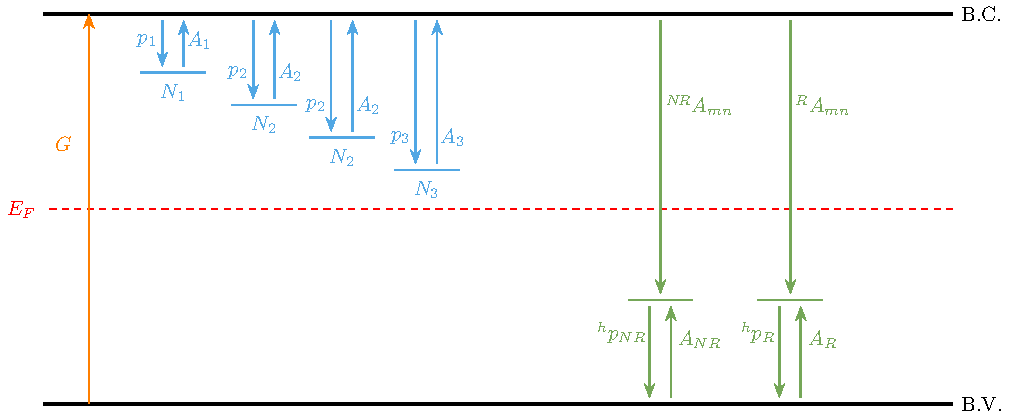
\includegraphics[width=\textwidth]{Images/modeldiagram.pdf}
  \caption[Jab\l oński diagram illustrating the theoretical TL model with traps and transitions.]{Jab\l oński diagram of the theoretical model for the thermoluminescence process. The energy is situated in the Y axis, and the different components of the system are shown: traps ($p_k$: electron release probability, $A_k$: recombination probability, $N_k$: total density of available positions), recombination centers ($^hp_j$: hole excitation probability, $A_j$: electron trapping probability, $^jA_{mn}$: electron recombination probability), and the conduction (C.B) and valence (V.B) bands with the respective electron-hole pair generation rate ($G$).}
  \label{fig:TheoreticalModel}
\end{figure}

\vspace{10pt}
The introduction of impurities or defects however, break the periodicity of the lattice, and create localized energy levels inside this ``forbidden region''. These levels can be thought of as traps for electrons if we are situated above the fermi level, and traps of holes if we are situated below. When this material is irradiated, electrons from the valence band can be excited to the conduction band, creating an electron-hole pair; and so changing the shape of the occupancy function. Once excited, both electrons and holes get ``trapped'' in these localized energy levels, and the excitation of these pairs into equilibrium will result in the emission of energy. In Figure \ref{fig:FD_irradiation} we can see a broad description of the perturbation of the system from its equilibrium state due to the irradiation, and the return of the system to equilibrium during either thermal stimulation or optical stimulation. If said relaxation processes are radiative, TL and OSL result. 

\vspace{10pt}

And so, we can see a schematic representation of our theoretical model in Figure \ref{fig:TheoreticalModel}. Situating the energy in the Y axis, the focus is set in the energy gap of our material. Drawn as a blue or green horizontal line are the energy traps; in blue above the Fermi level there are electron traps, and in green there are ``hole traps'' or recombination centers. The vertical arrows describe available transitions; the ones pointing upwards represent an excitation process, and the ones pointing downwards represent a relaxation process. 

\vspace{10pt}

Mathematically, we can describe these processes with a set of differential equations that take into account the rate of change of the number of electrons and holes in the bands and traps. This set will depend on the properties of the material, and the luminescence response we are trying to model. For an arbitrary system, we can write the following set of equations that describe the rate of change of the number of electrons and holes in the conduction band $n_c$, the valence band $n_v$:
\vspace{10pt}

\begin{equation} \label{eq:dn_cdt}
  \frac{dn_c}{dt} = \textcolor{orange}{G} - \textcolor{customblue}{\left[\sum_i \frac{dn_i}{dt}\right]} \cdot n_c - \textcolor{customgreen}{\left[ \sum_{j=R, N\!R}\, ^jA_{mn} \cdot m_j \right]} \cdot n_c
\end{equation}

\begin{equation} \label{eq:dn_idt}
  \textcolor{customblue}{\frac{dn_i}{dt} = -p_i \cdot n_i + A_i \cdot [N_i - n_i]}
\end{equation}

\begin{equation} \label{eq:dm_jdt}
  \textcolor{customgreen}{\frac{dm_j}{dt} = -^hp_j \cdot m_j + A_j \cdot [M_j - m_j]} \cdot n_v - \textcolor{customgreen}{^iA_{mn} \cdot m_j} \cdot n_c
\end{equation}

\begin{equation} \label{eq:dn_vdt}
  \frac{dn_v}{dt} = \textcolor{orange}{G} - \textcolor{customgreen}{\sum_{j=R, N\!R} \left[-^hp_j \cdot m_j + A_j \cdot [M_j - mj] \textcolor{black}{~ \cdot ~n_v}\right]} 
\end{equation}

\vspace{15pt}
Where every term is defined as follows:
\begin{itemize}[itemsep=0.2cm,parsep=0cm]
  \item $G$: electron-hole pairs generation rate by the radiation [cm$^{-3}$ s$^{-1}$]
  \item $n_c$: electron concentration in the conduction band [cm$^{-3}$]
  \item $n_v$: electron concentration in the valence band [cm$^{-3}$]
  \item $n_i$: electron concentration in trap i [cm$^{-3}$]
  \item $m_j$: hole concentration in the recombination center j [cm$^{-3}$]
  \item $N_i$: total density of available positions in trap i [cm$^{-3}$]
  \item $M_j$: total density of available positions in recombination center j [cm$^{-3}$]
  \item $p_i$: electron release probability factor for trap i [s$^{-1}$]
  \item $^hp_j$: hole release probability factor for recombination center j [s$^{-1}$]
  \item $A_i$: electron trapping probability factor for trap i [cm$^{3}$ s$^{-1}$]
  \item $^jA_{mn}$: recombination probability factor for recombination center j [cm$^{3}$ s$^{-1}$]
\end{itemize}

\vspace{10pt}

Equation \ref{eq:dn_cdt} describes the change rate of electron concentrations in the conduction band. To interpret this equation, we can see that to the electron-hole pairs generated by the radiation ($G$), there are two terms subtracted. The first one correlates to the electrons that leave the continuum levels of the conduction band and get trapped in the discrete levels of the material ---a process described by \ref{eq:dn_idt}, that will have a further discussion in section \ref{sec:factorfrecuencia}---, and the second one answers to the electrons in the conduction band that recombine with holes with a radiative ($R$) or non-radiative ($N\!R$) process. It is easy to see that this second term corresponds to the third term of \ref{eq:dm_jdt}. 

\vspace{10pt}
The change rate of electron concentrations in the valence band is shown in \ref{eq:dn_vdt}, and it follows a similar logic. This time however, we only take into account the terms multiplied by the electron density in the valence band ($n_v$) seen in equation \ref{eq:dm_jdt}; one that represents the holes leaving the continuum to get trapped in the recombination centers, and another that accounts for the addition of electrons that are released from the recombination centers and recombine with the holes in the valence band. The terms described correspond to Equations \ref{eq:dn_idt} and \ref{eq:dm_jdt} describe the total change rate of electrons and holes in the discrete levels of the material. The signs of the terms in these equations follow the convention that we are set in the conduction band, and so any electron that leaves the conduction band is represented with a negative term, and any electron that enters is represented with a positive term.

\vspace{10pt}

To carry out a numerical simulation of the process, we will need to solve the set of differential equations \ref{eq:dn_cdt} -- \ref{eq:dn_vdt} using RKF-45 method, which is a Runge-Kutta method of order 4 and 5. This method will obtain the charge concentration in all traps and recombination centers at an instant of time. The solving of this set of equations will be done for the three phases required to obtain the TL glow curve. To do this, the intrinsic and kinetic parameters are kept constant, varying the external conditions of the system such as temperature and electron-hole pair generation rate. 

\vspace{10pt}
The first phase is \textit{irradiation}, where the material is exposed to ionizing radiation. It begins with all levels initially empty [$n_c(0) = n_v(0) = n_i(0) = m_j(0) = 0$], and the electron-hole pairs generated as a result will have a constant value as a function of time ($G = 1000$ cm$^{-3}$ s$^{-1}$). The temperature is set to a constant $T = 25$ \textdegree C and the filling process takes one hour (3600 seconds). The second phase is \textit{relaxation}, where the material is left undisturbed at a constant temperature for a defined period of time. Taking as initial values the final values of the irradiation phase, the temperature is kept constant at $T = 25$ \textdegree C, and the electron-hole pairs generation rate is set to $G = 0$ cm$^{-3}$ s$^{-1}$. The relaxation process is set for one week (604,800 seconds). Finally, the third phase is \textit{heating}, where the material is taken from an initial temperature $T_0$ to a final temperature at a constant linear heating rate during 400 seconds. The numerical resolution of the set equations is similar to the previous phases, but now with the temperature varying linearly with the expression:

\begin{equation} \label{eq:heating}
  T(t) = T_0 + \beta \cdot t
\end{equation}

\vspace{7pt}
Where the heating rate is set to $\beta = 1 $ \textdegree C s$^{-1}$. The electron-hole pairs generation rate is set to $G = 0$ cm$^{-3}$ s$^{-1}$, and the charge concentration values are taken from the final values of the relaxation phase. The heating process is set to last 400 seconds. The results after the numerical resolution of the set of equations will be the charge concentration values for every instant of time throughout the whole heating cycle [$n_c(t), n_v(t), n_i(t), m_j(t)$]. It is in this phase when the luminescent emission occurs, and so the intensity of the emitted light can be estimated in relation to the radiative recombination of electron-hole pairs. We can give the expression for the intensity of the emitted light as it follows:

\begin{equation} \label{eq:intensity}
  I_{T\!L}(t) = -\frac{dm}{dt} \approx {}^RA_{mn} \cdot m_R \cdot n_c
\end{equation}

\vspace{7pt}

We can write this dependence as a function of temperature by:

\begin{equation}
  I_{T\!L}(t) = -\frac{dm}{dt} = -\frac{dm}{dt} \cdot \frac{dT}{dT} = -\frac{dm}{dT} \cdot \frac{dT}{dt} = -\frac{dm}{dT} \cdot \beta = I_{T\!L}(T) \cdot \beta
\end{equation}

Representing this intensity as a function of temperature will be the objective of the simulations, as it is the key to understand the thermoluminescent response of the LiF:Mg,Ti after being irradiated.

\section{Analysis of the electron release probability} \label{sec:factorfrecuencia}

As introduced in Section \ref{sec:modelo}, there is a greater discussion to be had about the releasing probability of electrons and holes, as it determines in great part the electron-hole pairs available to recombine. In general, two distinct mechanisms may contribute to the release of a trapped carrier: \textit{thermal} and \textit{optical (photo)excitation}. In the first one, the electron gains sufficient energy from lattice vibrations to overcome the trap depth, and in the latter the release is induced by the absorption of a photon whose energy exceeds the one binding the carrier to the trap. An electron trapped in a lattice defect with energy $E_t$ and temperature $T$ will have a probability of being released that is the result of:

\begin{equation}
  p = p_{th} + p_{ph}
\end{equation}

Where $p_{th}$ is the thermal excitation probability and $p_{ph}$ is the optical excitation probability. The thermal contribution follows Arrhenius equation. The probability per unit of time that the electron will be thermally excited into the conduction band is given by:

\begin{equation} \label{eq:p_th}
  p_{th} = s \cdot e^{-\frac{E_t}{k_B T}}
\end{equation}

\vspace{10pt}
Where $s$ is known as the \textit{frequency factor} [s$^{-1}$]. It can be interpreted as the ``attempt to escape'' frequency, as it is a measure of the number of times per second that energy is absorbed from phonons in the lattice. The exponential that follows is the probability that the energy absorbed is enough to cause a transition from the localized state to the conduction band. For the optical contribution on the other hand, the trapped electrons are released from their traps via absorption of energy from photons \cite{mckeever_course_2022}, and the probability is given by:

\begin{equation}
  p_{\text{ph}} = \sigma_P(E) \cdot \Phi
\end{equation}

Where $\sigma_P(E)$ is the photoionization cross-section [cm$^2$], which is a measure of the probability that a photon with energy $E$ will be absorbed by an electron trapped in a lattice defect, and $\Phi$ is the photon flux or intensity of the stimulating light [cm$^{-2}$ s$^{-1}$], which is the number of photons per unit area per unit time. This process is particularly relevant in optically stimulated luminescence (OSL), where the material is stimulated with light to release the trapped electrons and produce a luminescent signal. If $E_0$ is the threshold photon energy required to excite the electron from the trap, instead of considering only the thermal trap depth $E_t$ as one may expect, we should initially consider the effect of the contribution of lattice phonons such that:

\begin{equation}
  E_0 = E_t + E_{ph}
\end{equation}

Where $E_{ph}$ is given by:

\begin{equation}
  E_{ph} = S_{H\!R} \cdot h \cdot \nu_{ph}
\end{equation}

\vspace{7pt}

And here $S$ is the Huang-Rhys factor, which is a dimensionless parameter that characterizes the degree of electron-phonon coupling in a luminescent material that usually ranges on the order of 1--2 \cite{mckeever_1995}. The higher the Huang-Rhys factor, the stronger the electron-phonon coupling, and so the greater the energy shift of the trap level due to lattice vibrations. The term $h \cdot \nu_{ph}$ is the phonon energy with frequency $\nu_{ph}$ [s$^{-1}$], where $h$ is Planck's constant [eV $\cdot$ s]. For LiF the phonon frequency is typically around 900 cm$^{-1}$ \cite{bransden_atomics}, which corresponds to a phonon energy of approximately 0.11 eV. If we take a Huang-Rhys factor of $S_{HR} = 1$, we can estimate the energy shift given a set of experimental values for the thermal energies $E_t$ of the traps. The results are shown in \ref{tab:energythresholds} and with them we see that the energy threshold $E_0$ is primarily determined by the thermal trap depth $E_t$, with the phonon energy $E_{ph}$ contributing a small correction.

\renewcommand{\arraystretch}{1.5}
\begin{longtable}[c]{lllll}
\caption[Energies for the different traps and recombination centers in LiF:Mg,Ti.]{Energies for the different traps and recombination centers in LiF:Mg,Ti. $E_t$ represents the thermal energy, $E_{ph}$ the phonon energy, and $E_0$ the total energy threshold.}
\label{tab:energythresholds}\\
\hline
\multicolumn{2}{l}{Parameters}                            & $E_t$ (eV) & $E_{ph}$ (eV) & $E_0$ (eV) \\ \hline
\endhead
\hline
\endfoot
\endlastfoot
\multirow{6}{*}{Trapping Centers}      & Trap I        & 1.19       & 0.11         & 1.30       \\
                                       & Trap II       & 1.60       & 0.11         & 1.71       \\
                                       & Trap III      & 1.76       & 0.11         & 1.87       \\
                                       & Trap IV       & 1.87       & 0.11         & 1.98       \\
                                       & Trap V        & 1.98       & 0.11         & 2.09       \\
                                       & Trap s        & 2.70       & 0.11         & 2.81       \\ \hline
\multirow{2}{*}{Recombination centers} & Radiative     & 2.30       & 0.11         & 2.41       \\
                                       & Non Radiative & 2.30       & 0.11         & 2.41       \\ \hline
\end{longtable}

\vspace{10pt}

This observation reinforces the suitability of studying the TL independently of optically stimulated luminescence (OSL). The fact that the thermal energy $E_t$ stays over zero confirms that thermal energy alone is sufficient to release charge carriers from traps over a physically accessible temperature range. Furthermore, in TL measurements, no external optical stimulation is applied during readout, and so the photon flux in a darkened environment is negligible. As a result, photo-induced excitation does not contribute meaningfully to the observed luminescence signal. From now on, we will close our focus on the thermoluminescence process, and so we will only consider the thermal excitation probability $p_{th}$ in our simulations.

\vspace{10pt}

If we aim to deepen our understanding of equation \ref{eq:p_th}, we can look a little further in the concept of the frequency factor $s$. It is a crucial parameter in the study of thermoluminescence, as it determines the rate at which electrons are released from traps. It is a function of the material properties, as shown in its definition:

\begin{equation} \label{eq:freqfactor}
  s = \nu_{ph} \cdot K \cdot e^{\frac{\Delta S}{k_B}}
\end{equation}

\vspace{10pt}
Where $\nu_{ph}$ is the lattice phonon vibration frequency and $K$ is the transition probability constant, that takes the value 0 or 1 depending on whether the transition is allowed or forbidden. Typically, one can expect $s \sim 10^{12} -10^{14}$ s$^{-1}$, which is consistent with the values of $\nu$ for most solids. The term $e^{\nicefrac{\Delta S}{k_B}}$ is a correction factor that accounts for the entropy change associated with the transition from the localized state to the conduction band. 

\vspace{10pt}

From equation \ref{eq:freqfactor} we see that the frequency factor has an exponential dependency with the entropy change. This, taking the Quantum Statistical Mechanics theory \cite{brey}, does not align with the invariance of said factor with temperature, as entropy, with its own definition, should vary when temperature does. While a rigorous proof of the overall temperature dependence of the frequency factor is beyond the scope of this work, one model is proposed to provide an approximate perspective on how this dependency could influence the resulting TL glow curve. 

\vspace{10pt}

At first glance, the simplest model was considered, where the entropy would be linear with the temperature ($\Delta S \propto T$). This theory was quickly discarded as would make the entropy factor increase exponentially with the temperature ($s \propto e^T$), and so the probability of excitation would tend to infinity in a very short range of temperature increase.

\vspace{10pt}

To solve this issue, a more refined model was considered, where the entropy would now be logarithmically dependent on the temperature ($\Delta S \propto \ln(T)$). The constant of the proportionality could be called $\alpha$, and so the resulting expression of the frequency factor can be written as:

\begin{equation}\label{eq:freqfactor_lnT}
    s = \nu_{ph} \cdot K \cdot T^{\nicefrac{\alpha}{k_B}}
\end{equation}

\vspace{10pt}

It is clear now that a softer dependency with the temperature is achieved, and the previous problem of the entropy factor tending to infinity is solved. The value of $\alpha$ can be adjusted to keep the entropy contribution at a realistic magnitude ---typically we have $\Delta S \sim  1\!-\!3 ~~k_B$ over the glow curve temperature range---. For that reason, we have selected a value of:

\begin{equation}
    \alpha = \frac{1.5 ~k_B}{ln(300)} \approx 0.26 ~k_B
\end{equation}

\vspace{10pt}

This choice ensures that the frequency factor remains within a reasonable range across the temperature spectrum of interest, and yields TL glow curves that are consistent with experimental observations of LiF:Mg,Ti materials.


\section{About LiF:Mg,Ti} \label{sec:LiF}


Lithium fluoride (LiF) is a crystalline material that has been widely used in radiation dosimetry due to its favorable % !!!!
properties. It first appeared as a thermoluminescent dosimetry material in the 1950's, and since then, it has been extensively studied in the field of radiation detection. The material is composed of lithium (Li) and fluor (F) %?????
atoms, forming a crystal lattice structure of a face-centered cubic (FCC) type. Without any impurities, LiF is a semiconductor, with a bandgap of approximately 14 eV, which makes it an excellent insulator at room temperature.

\vspace{10pt}

To enhance the properties for radiation detection, LiF is often doped with magnesium (Mg) and titanium (Ti) ions, and sold commercially as TLD-100 \cite{horowitz_thermoluminescence_2007}. The doping process introduces defects in the crystal lattice, creating energy levels within the bandgap. These defects play a crucial role in trapping and releasing charge carriers, which are responsible for the thermoluminescent response of the material. This process is known as thermoluminescence, where the trapped electrons are released upon heating, resulting in the emission of light. The intensity of this emitted light is proportional to the amount of radiation absorbed by the material, making it a valuable tool for dosimetry.

\vspace{10pt}

The TL response of LiF:Mg,Ti is characterized by a glow curve, which is a plot of the intensity of emitted light as a function of temperature. The glow curve typically exhibits several peaks, each corresponding to different trapping levels in the material. The position and shape of these peaks can provide valuable information about the trapping and recombination processes occurring in the material, and they are key to understanding the thermoluminescent response of LiF:Mg,Ti. In Figure \ref{fig:ExperimentalGlowCurve} we can see an experimental glow curve of LiF:Mg,Ti plotted with data provided by the Radiation Dosimetry Laboratory of CIEMAT, which shows a typical response with several peaks at different temperatures. 

\begin{figure}[ht]
    \centering
    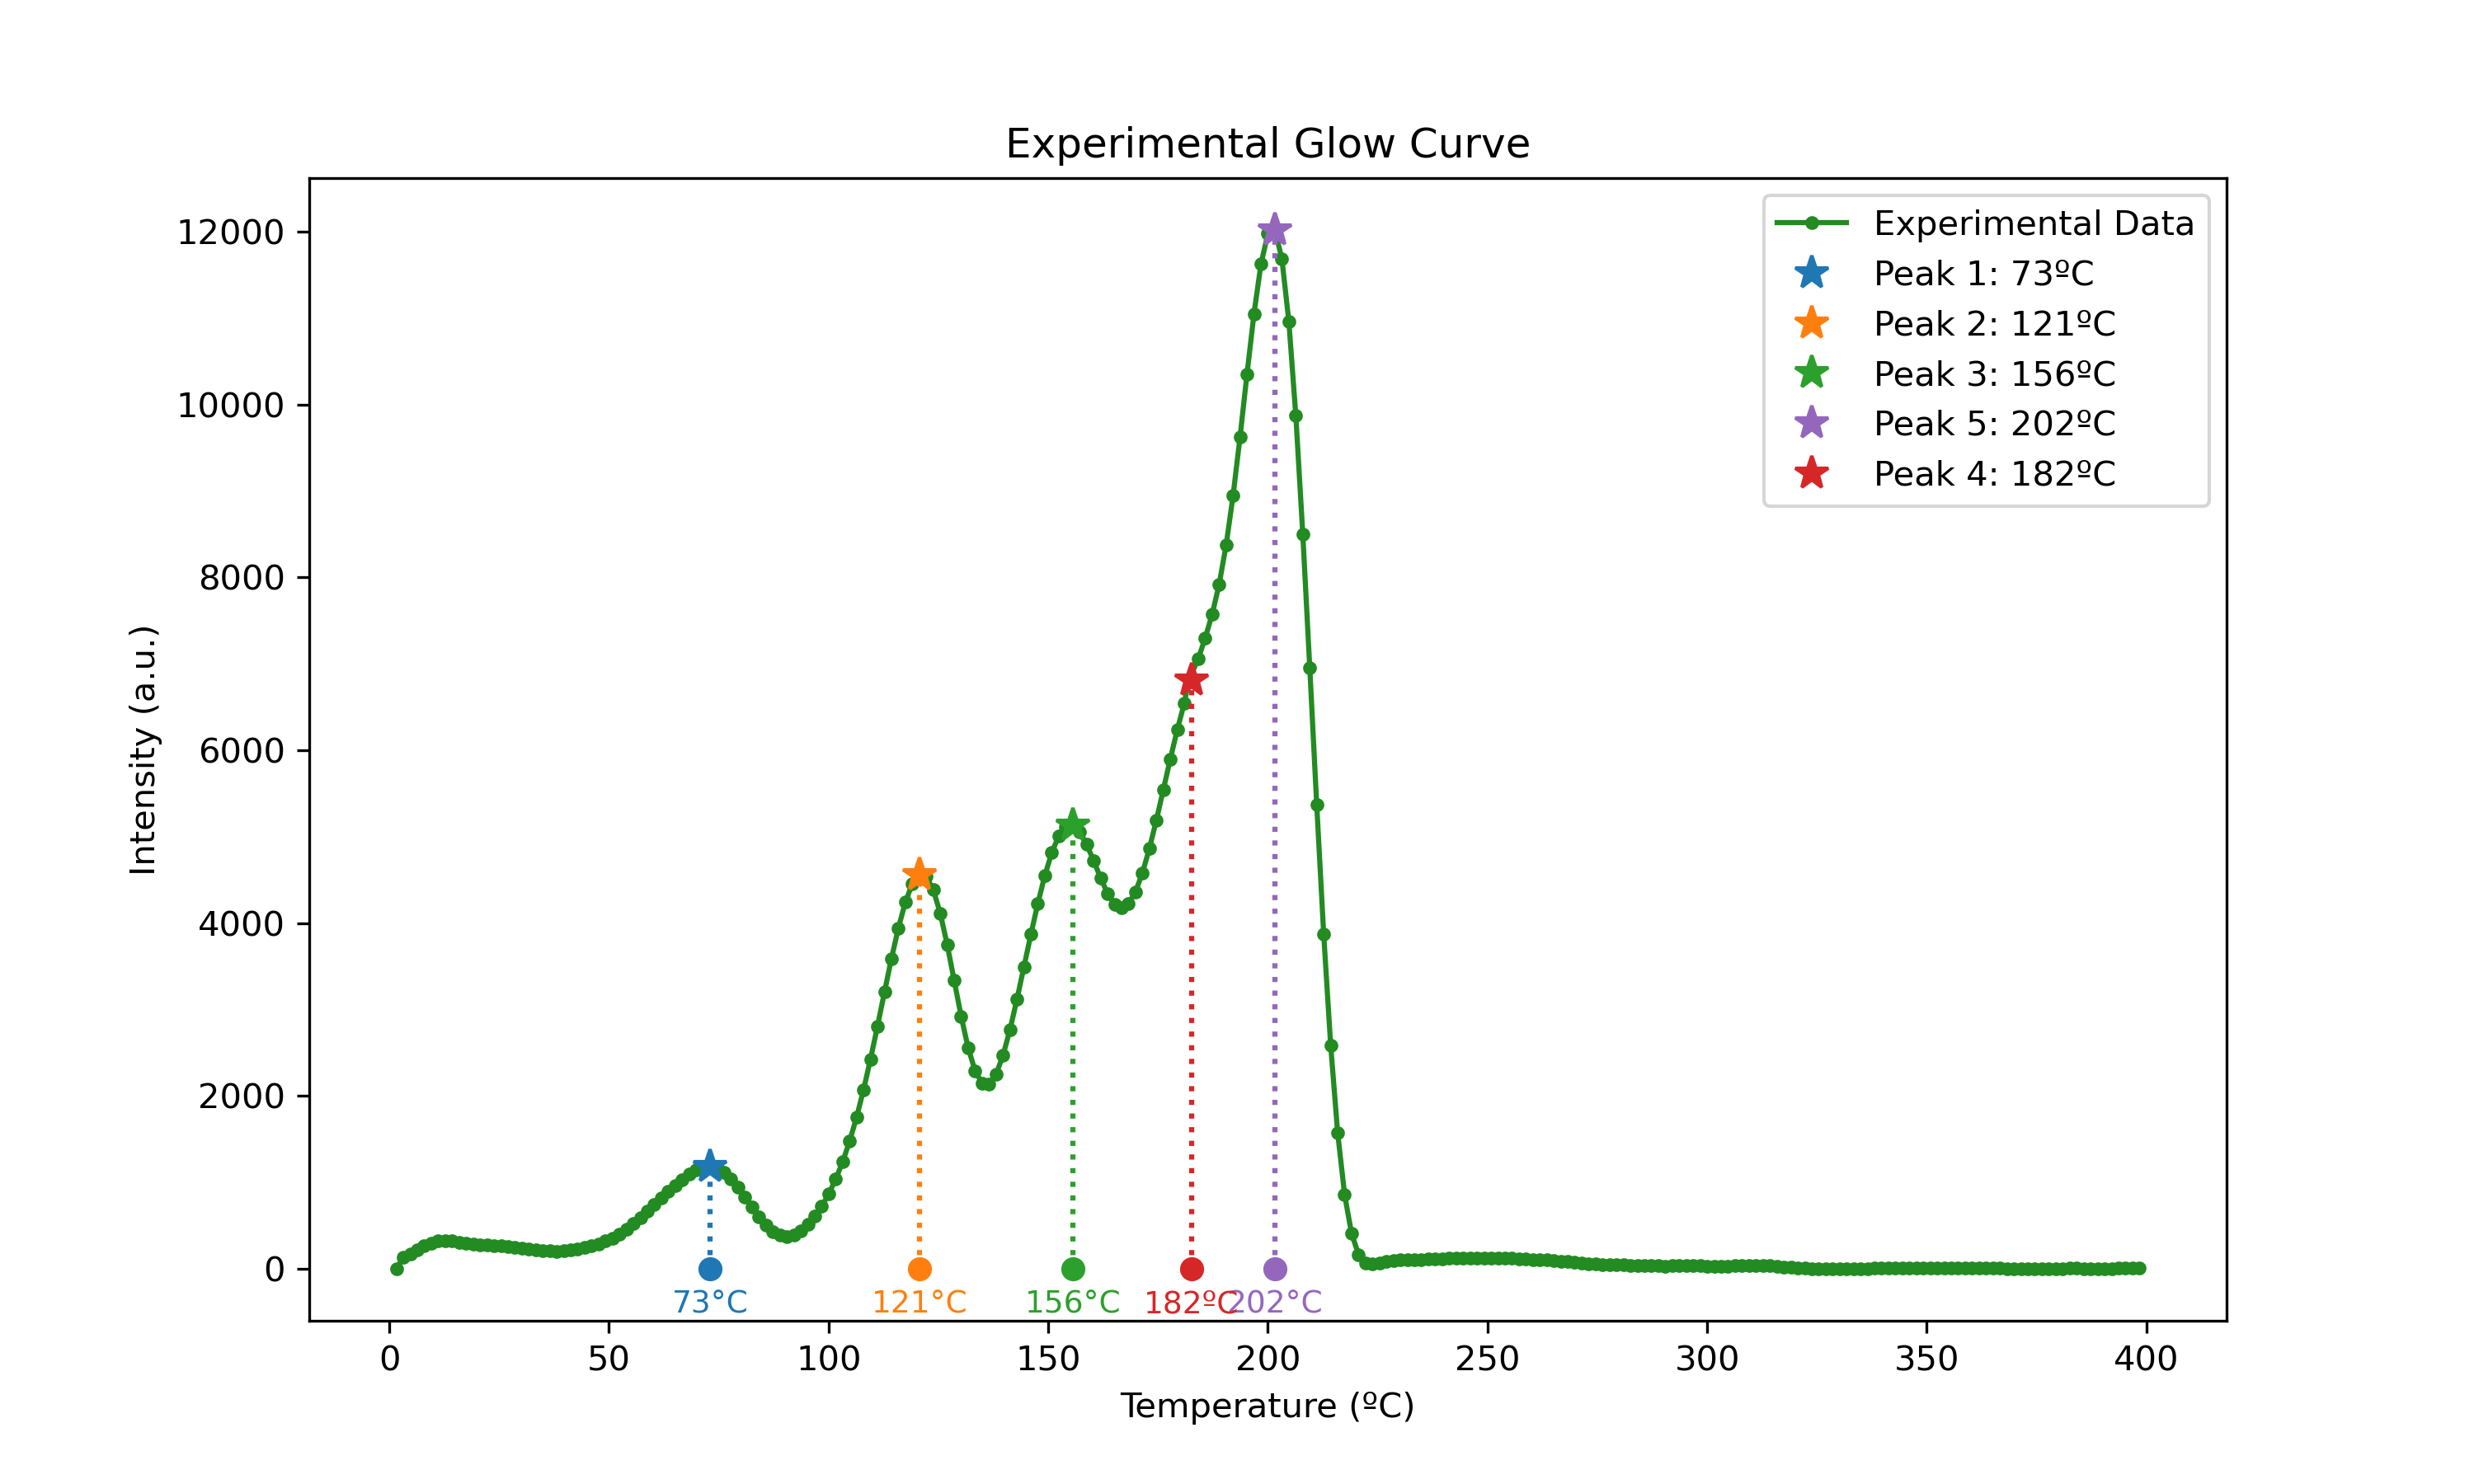
\includegraphics[width=\textwidth]{Images/Experimental_Glow_Curve.png}
    \caption[Experimental TL glow curve of LiF:Mg,Ti.]{Experimental thermoluminescence glow curve of LiF:Mg,Ti showing the emitted light intensity [u.a] plotted against temperature (\textdegree C). The most prominent is the main dosimetric peak around 200 \textdegree C, which is stable and reproducible. Lower-temperature peaks (<150 \textdegree C) correspond to shallow traps with poor thermal stability, while intermediate peaks (150–200 \textdegree C) suggest more complex trapping mechanisms. The measurement reflects the material’s characteristic response following exposure to ionizing radiation.}
    \label{fig:ExperimentalGlowCurve}
\end{figure}
\vspace{10pt}

This characteristic shape of the glow curve for LiF:Mg,Ti has been extensively documented \cite{mckeever_course_2022} \cite{benavente_LiF} \cite{massillon-jl_role_nodate}, and it is a result of the specific energy levels introduced by the doping process, with the main peak typically occurring around 200 \textdegree C. Each peak arises from the thermal release of electrons from traps of different activation energies, if followed by recombination in the recombination centers. The graph shows the luminescence intensity plotted against temperature, and reveals five distinct glow peaks. Each of those peaks corresponds to the thermal release of trapped charge carriers from specific trap levels, and their height and position can be crucial to determine the trap depth and recombination probability. They can be categorized into:

\begin{itemize}
  \item \textbf{Main dosimetric peak ($\sim$ 200 \textdegree C).} It has the most favorable characteristics for dosimetry: high intensity, good linearity with dose, and appears consistency at the same temperature, which helps to exhibit good reproducibility across different measurements and a relatively simple kinetic behavior. It is thermally stable at room temperature for long periods of time, meaning their signal do not fade significantly over days or weeks. 
  \item \textbf{Lower-temperature peaks (< 150 \textdegree C).} They are associated with shallower traps, and are thermally less stable at ambient conditions. They tend to fade significantly at room temperature over time ---that is, undergo great signal loss due to thermal stimulation from room temperature alone---, and as a consequence, are not useful for dosimetric purposes. However, they are useful for fundamental studies of trapping and recombination processes, offering insight into the energy structure of the material and their mechanisms of carrier release. 
  \item \textbf{Intermediate peaks (between 150 \textdegree C and 200 \textdegree C).} As expected, they suppose a middle ground. These peaks represent a transitional region in trap stability and interaction complexity. They are believed to arise from more complex or composite trapping structures, possibly involving multiple trapping levels or interactions between traps and recombination centers and their intensity and position can shift or merge depending on the specific conditions of the sample, the dose or the thermal history. In some cases, peaks in this range can interfere with or overlap the main dosimetric peak, which can complicate deconvolution and dose evaluation.
\end{itemize}

\chapter{Simulations} \label{ch:4}

\section{Tools and software used for simulations} \label{sec:materials}

The materials used for this work are all the digital tools required for the simulation of the behavior of our material of choice. In our case, the project was made using \textit{Python} in a Jupyter Notebook. The programs written are available on the GitHub repository called \href{https://github.com/MartadelaRosa/TFG_MartadelaRosa}{\texttt{TFG\_MartadelaRosa}}. 

\vspace{10pt}

The libraries used for the simulations are:
\begin{itemize}
    \item \texttt{numpy}: This library is used for numerical calculations and array manipulations.
    \item \texttt{matplotlib}: This library is used for plotting graphs and visualizing data.
    \item \texttt{pandas}: This library is used for data manipulation and analysis, providing data structures like DataFrames.
    \item \texttt{scipy}: This library is used for scientific computing and includes functions for optimization, integration, interpolation, and more. In particular to solve the differential equations that describe the kinetics of the TL process.
\end{itemize}



\section{Simulations} \label{sec:simulations}

To compute a simulation of the TL process described in Section \ref{sec:modelo}, after defining the parameters of the model, we need to solve the differential equations that describe the kinetics of the TL process. The equations are solved using the \texttt{odeint} function from the \texttt{scipy.integrate} library. The function takes as input the system of equations, the initial conditions, and the time points at which we want to evaluate the solution. The output is an array containing the values of the variables at each time point, which is then saved to their corresponding variables, used to plot the results. They are brought to life using the \texttt{matplotlib} library, and for every resolution of the differential equations, we will present three graphs as the result.

\vspace{10pt}

The first step to perform the simulations is to define the parameters of the model. These parameters include the activation energy ($E_i$), the frequency factor ($s_i$), the electron trapping probability factor ($A_i$), and total density of electrons ($N_i$) for each trapping center, as well as the recombination centers. The parameters used in our case can be found in Table \ref{tab:simulationparameters}. The values of these parameters are based on experimental data \cite{benavente_LiF} for the specific material being studied, in this case, LiF:Mg,Ti, and are proposed within the margin of error. Once the model parameters have been defined, the simulation proceeds by numerically solving the system of differential equations described in equations \ref{eq:dn_cdt}--\ref{eq:dn_vdt}. As we mentioned, this is done by using \texttt{odeint} function from the \texttt{scipy.integrate} library. For each phase, the appropriate parameters and initial conditions are set to a general simulation function that returns the evolution of all charge concentrations. 


\renewcommand{\arraystretch}{1.5}
\begin{longtable}[c]{llcccc}
\caption[Kinetic and structural parameters used in the simulations.]{Kinetic and structural parameters used in the simulations. Each trap and recombination center is characterized by its activation energy ($E_i$), frequency factor ($s_i$), electron trapping probability factor ($A_i$), and total density of electrons ($N_i$). The values are based on experimental data for LiF:Mg,Ti.}
\label{tab:simulationparameters}\\
\hline
\multicolumn{2}{l}{Parameters} & \multicolumn{1}{c}{E (eV)} & \multicolumn{1}{c}{s (s$^{-1}$)} & \multicolumn{1}{c}{A (cm$^3$ s$^{-1}$)} & \multicolumn{1}{c}{N (cm$^3$)} \\ \hline
\endhead
%
\hline
\endfoot
%
\endlastfoot
%
\multirow{6}{*}{Trapping Centers}      & Trap I        & 1.19   & 1.00 $\cdot 10^{15}$ &  $10^{-8}$ &  $10^{10}$ \\
                                       & Trap II       & 1.60   & 1.41 $\cdot 10^{14}$ &  $10^{-8}$ &  $10^{10}$ \\
                                       & Trap III      & 1.76   & 9.05 $\cdot 10^{15}$ &  $10^{-8}$ &  $10^{10}$ \\
                                       & Trap IV       & 1.87   & 5.78 $\cdot 10^{15}$ &  $10^{-8}$ &  $10^{10}$ \\
                                       & Trap V        & 1.98   & 8.71 $\cdot 10^{17}$ &  $10^{-8}$ &  $10^{10}$ \\
                                       & Trap s        & 2.70   & 1.00 $\cdot 10^{15}$ &  $10^{-8}$ &  $10^{10}$ \\ \hline
\multirow{2}{*}{Recombination centers} & Radiative     & 2.30   & 1.00 $\cdot 10^{16}$ &  $10^{-8}$ &  $10^{10}$ \\
                                       & Non Radiative & 2.30   & 1.00 $\cdot 10^{16}$ &  $10^{-8}$ &  $10^{10}$ \\ \hline
\end{longtable}

To ensure modularity and consistency, the simulation is structured in reusable components. Each phase is simulated by calling the same solver function with different input values, and the output is automatically stored and passed between stages as initial conditions to the next one to maintain continuity. As two models have been used for the simulations, two separate functions were created to define the system of differential equations for the TL process. The first function, \texttt{diff\_eqs\_freqfactor()}, is used for the simulations of the TL process with a frequency factor that depends on the temperature following equation \ref{eq:freqfactor_lnT}, while the second function, \texttt{diff\_eqs\_notemp()}, is used for the simulations where the frequency factor is a constant from Table \ref{tab:simulationparameters}. The functions take as input the current state of the system, the time, and the parameters of the model, and return the derivatives of the charge concentrations with respect to time. In the Listing \ref{lst:irradiation}, we can see the implementation of the first function for the irradiation phase of the TL process.

\vspace{10pt}

\renewcommand{\baselinestretch}{1}
\begin{lstlisting}[language=Python, caption={Python simulation of the irradiation phase in TL simulations. It defines the initial parameters, initializes trap and recombination center populations, solves the system of differential equations, and plots the results.}, label=lst:irradiation]

## 2.1 IRRADIATION
# Parameters for IRRADIATION
value.kB = 8.617e-5        # Boltzmann constant (eV/K)
value.T_C = 25             # Temperature (celsius)
value.hr = 0               # Heating rate (celsius/s)
value.G = 1000             # e-hole pair gen (cm-3 s-1)

# Time vector (s)
npoints = 3600
t = np.linspace(0, npoints-1, npoints)

# Initial conditions vector
n_I, n_II, n_III, n_IV, n_V, n_s = 0, 0, 0, 0, 0, 0
m_NR, m_R = 0, 0
n_c, n_v = 0, 0
y0 = [n_I, n_II, n_III, n_IV, n_V, n_s, m_NR, m_R, n_c, n_v]

# Solving the differential equations system
irradiation = odeint(diff_eqs_freqfactor, y0, t, args=(value,))
n_I, n_II, n_III ,n_IV ,n_V ,n_s ,m_R ,m_NR ,n_c , n_v 
    = irradiation.T

# Plotting the results
plot_results(irradiation, save_path, t, value)


\end{lstlisting}
\renewcommand{\baselinestretch}{1.5}

\vspace{10pt}

After solving the system of differential equations for a given phase, the simulation outputs three diagnostic plots that represent the state and evolution of the material over time (or temperature in the case of the \textit{heating} phase). These are:

\begin{itemize}
    \item \textbf{Electron concentration $\mathbf{n_i(t)}$ evolution:} This plot shows the temporal evolution in each trap. It provides insight into how the electron population in each trap changes over time, indicating the trapping and de-trapping processes. It shows how they are progressively filled with electrons during the irradiation phase, their stationary behavior in the relaxation phase, and their depletion during the heating phase. Their evolution depends on the parameters of each trap, and will have different shapes as a consequence.
    \item \textbf{Recombination rates:} The graph displays the rate of radiative ($dm_R$) and non-radiative ($dm_{NR}$) recombination processes as a function of time. It shows how the recombination rates change as the traps are filled and emptied. During irradiation, $dm_R$ grows steadily as the traps fill up, to then drop rapidly to near zero during the relaxation phase, indicating that radiative recombination ceases once the irradiation stops and the system stabilizes in a metastable state. During heating, $dm_R$ rises again as the trapped electrons are thermally released and recombine radiatively with holes, producing the TL glow peaks. It is in this graph for the heating phase when we expect to obtain out TL glow curve. Throughout all three phases, the non-radiative recombination rate ($dm_{NR}$) remains constant, confirming that non-radiative recombination plays an insignificant role in simulations.
    \item \textbf{Charge neutrality:} This plot shows the ratio of the total electron concentration to the total hole concentration as a function of time. It follows the expression:
    \begin{equation}
        \frac{n_c + n_I + n_{II} + n_{III} + n_{IV} + n_V + n_s}{m_R + m_{N\!R} + n_v} \approx 1
        \label{eq:charge_neutrality}
    \end{equation}
    And as such, it should be close to 1 throughout the simulation. This plot is useful to verify that the system remains charge neutral during the entire process, and can serve as a validity check to ensure that the simulation is correctly implemented. If the ratio deviates significantly from 1, it may indicate an error in the model or the numerical solution.
\end{itemize} 
\chapter{1}


\section{Primera sección}

At vero eos et accusamus et iusto odio dignissimos ducimus 
qui blanditiis praesentium voluptatum deleniti atque corrupti 
quos dolores et quas molestias excepturi sint occaecati cupiditate 
non provident, similique sunt in culpa qui officia deserunt mollitia animi, 
id est laborum et dolorum fuga. Et harum quidem rerum facilis est et expedita 
distinctio. Nam libero tempore, cum soluta nobis est eligendi optio cumque 
nihil impedit quo minus id quod maxime placeat facere possimus, omnis voluptas 
assumenda est, omnis dolor repellendus. Temporibus autem \cite{Bellomo2000} quibusdam et aut 
officiis debitis aut rerum necessitatibus saepe eveniet ut et voluptates 
repudiandae sint et molestiae non recusandae. Itaque earum rerum hic 
tenetur a sapiente delectus \cite{Arfken2005}, ut aut reiciendis voluptatibus maiores 
alias consequatur aut perferendis doloribus asperiores repellat.

\begin{equation}\label{eq:1a}
	\vec {a} = {\frac{{dv}}{{dt}}}\hat {u}_{T} + v{\frac{{d\hat{u}_{T} }}{{dt}}} = 
			   {\frac{{dv}}{{dt}}}\hat {u}_{T} + {\frac{{v^{2}}}{{\rho}} }\hat {u}_{N}
\end{equation}

Nam libero tempore, cum soluta nobis est eligendi optio cumque 
nihil impedit quo minus id quod maxime placeat facere possimus, omnis voluptas 
assumenda est, omnis dolor repellendus. Temporibus autem quibusdam et aut 
officiis debitis aut rerum necessitatibus saepe eveniet ut et voluptates 
repudiandae sint et molestiae non recusandae.

\begin{equation*}
	E = 4\varepsilon \left[ \left( \frac{\sigma}{r} \right)^{12} -
							\left( \frac{\sigma}{r} \right)^{6} \right]
\end{equation*}
			
\subsection{Primera subsección}

At vero eos et accusamus et iusto odio dignissimos ducimus 
qui blanditiis praesentium voluptatum deleniti atque corrupti 
quos dolores et quas molestias excepturi sint occaecati cupiditate 
non provident, similique sunt in culpa qui officia deserunt mollitia animi, 
id est laborum et dolorum fuga. Et harum \eqref{eq:1a} quidem rerum facilis est et expedita 
distinctio. Nam libero tempore, cum soluta nobis est eligendi optio cumque 
nihil impedit quo minus id quod maxime placeat facere possimus, omnis voluptas 
assumenda est, omnis dolor repellendus. 

\begin{figure}[H]
  \centering
  
\includegraphics[width=3cm]{logo_ciencias.png}
  \caption{Pie de figura}
  \label{fig:ejemplo1}
\end{figure}

Temporibus autem quibusdam et aut 
officiis debitis aut rerum necessitatibus saepe eveniet ut et voluptates 
repudiandae sint et molestiae non recusandae. Itaque earum rerum hic 
tenetur a sapiente delectus, ut aut reiciendis voluptatibus maiores 
alias consequatur aut perferendis doloribus asperiores repellat.


\subsubsection{Primera subsubsección}

At vero eos et accusamus et iusto odio dignissimos ducimus 
qui blanditiis praesentium voluptatum deleniti atque corrupti 
quos dolores et quas molestias excepturi sint occaecati cupiditate 
non provident, similique sunt in culpa qui officia deserunt mollitia animi, 
id est laborum et dolorum fuga. Et harum quidem rerum facilis est et expedita 
distinctio. Nam libero tempore, cum soluta nobis est eligendi optio cumque 
nihil impedit quo minus id quod maxime placeat facere possimus, omnis voluptas 
assumenda est, omnis dolor repellendus. Temporibus autem quibusdam et aut 
officiis debitis aut rerum necessitatibus saepe eveniet ut et voluptates 
repudiandae sint et molestiae non recusandae. Itaque earum rerum hic 
tenetur a sapiente delectus, ut aut reiciendis voluptatibus maiores 
alias consequatur aut perferendis doloribus asperiores repellat.




\section{Segunda sección}

At vero eos et accusamus et iusto odio dignissimos ducimus 
qui blanditiis praesentium voluptatum deleniti atque corrupti 
quos dolores et quas molestias excepturi sint occaecati cupiditate 
non provident, similique sunt in culpa qui officia deserunt mollitia animi, 
id est laborum et dolorum fuga. 

\begin{table}[H]
\centering
    \begin{tabular}{lrr}
      \hline
      Valor & 1992-93 & 2002-03 \\
      \hline
      Blah & x & y \\
      Blah & x & y \\
      Blah & x & y \\
      \hline
    \end{tabular}
  \caption{Una tabla}
\end{table}




Et harum quidem rerum facilis est et expedita 
distinctio. Nam libero tempore, cum soluta nobis est eligendi optio cumque 
nihil impedit quo minus id quod maxime placeat facere possimus, omnis voluptas 
assumenda est, omnis dolor repellendus. Temporibus autem quibusdam et aut 
officiis debitis aut rerum necessitatibus saepe eveniet ut et voluptates 
repudiandae sint et molestiae non recusandae. Itaque earum rerum hic 
tenetur a sapiente delectus, ut aut reiciendis voluptatibus maiores 
alias consequatur aut perferendis doloribus asperiores repellat.


% .......

\chapter*{Conclusiones}
\addcontentsline{toc}{chapter}{Conclusiones}

En este trabajo se ha desarrollado, simulado y analizado un modelo matemático para la respuesta termoluminiscente (TL) del material LiF:Mg,Ti, de acuerdo con los objetivos planteados en el Capítulo \ref{ch:2}.

\vspace{10pt}

Primero, los procesos físicos detrás de la termoluminiscncia se tradujeron en un sistema de ecuaciones diferenciales capaz de describir el comportamiento del material siguiendo una serie de aproximaciones. A partir de esta base se desarollaron dos modelos diferentes, que se bifurcan en función de la expresión del factor de frecuencia; un primer modelo, el más simple y usado como referencia, asume un valor constante específico para cada trampa (ecuación \ref{eq:freqfactor}), y un segundo modelo que incorpora una dependencia de la temperatura en el factor de frecuencia basada en la mecánica estadística cuántica (ecuación \ref{eq:freqfactor_lnT}).

\vspace{10pt}

Ambos modelos han sido implementados en un entorno de simulación numérica que es capaz de solucionar el sistema de ecuaciones diferenciales para las tres fases claves del proceso termoluminiscente: irradiación, relajación y calentamiento. Las simulaciones han conseguido imitar el proceso de llenado de las trampas durante la irradiación (Figura \ref{fig:irradiation_nievolution}), la consecuente liberación de electrones en la fase de relajación (Figura \ref{fig:relaxation_nievolution}), y la liberación térmica final de electrones durante la fase de calentamiento (Figura \ref{fig:GC_ActivationAndPeakTemperatures}). La curva de brillo termoluminiscente obtenida para ambos modelos es consistente con la forma característica del comportamiento experimental del LiF:Mg,Ti (Figura \ref{fig:ExperimentalGlowCurve}). Los resultados han sido validados mediante un gráfico de prueba (Figuras \ref{fig:irradiation_chneutrality}, \ref{fig:relaxation_chneutrality} y \ref{fig:heating_chneutrality}) realizado para cada fase, que asegura que el sistema se mantiene eléctricamente neutro.

\vspace{10pt}

Tras comparar los resultados de ambos modelos, se ha demostrado que el modelo dependiente de la temperatura es capaz de describir mejor el comportamiento de la trampa I, ya que muestra una saturación más rápida durante la irradiación, una disminución más pronunciada en la densidad de electrones durante la relajación y una recombinación más temprana en la fase de calentamiento. También se observa un ligero desplazamiento en la posición e intensidad de los picos en la curva de brillo termoluminiscente (Figura \ref{fig:heating_TLGlowCurve}). Las trampas más profundas, de II a V, exhiben un comportamiento similar en ambos modelos, lo que indica que sus energías de activación, al ser más altas, hacen que sean menos sensibles a la dependencia de temperatura del factor de frecuencia.

\vspace{10pt}

Las curvas de brillo termoluminiscente simuladas (Figura \ref{fig:heating_TLGlowCurve}) son bastante similares a los datos experimentales. El gráfico muestra sus cinco picos característicos, cada uno coincidiendo con las temperaturas de activación y pico identificadas en los gráficos de evolución de $n_i(t)$. Esta estrecha correspondencia entre la temperatura de máxima liberación de cada trampa en la Figura \ref{fig:GC_ActivationAndPeakTemperatures} y su pico luminescente en la Figura \ref{fig:heating_TLGlowCurve}, confirma que los picos de intensidad reflejan de manera fiable las energías de activación de las trampas y sus probabilidades de recombinación.

\vspace{10pt}

En resumen, este estudio no solo reproduce el comportamiento termoluminiscente visto experimentalmente en el LiF:Mg,Ti mediante simulación por ordenador, sino que también demuestra que la introducción de una dependencia de la temperatura en el factor de frecuencia puede mejorar la capacidad del modelo para explicar la dinámica de los portadores de carga involucrados en el proceso. Estos hallazgos subrayan la importancia del sutil efecto de la temperatura en el modelado termoluminiscente, y abren camino para futuros trabajos que refinen aún más el modelo, potencialmente incorporando una dependencia de temperatura más compleja. El contenido de este Trabajo Fin de Grado se presentará en la 51ª Reunión Anual de la Sociedad Nuclear Española el 24 de septiembre de 2025.


\chapter*{Conclusions}
\addcontentsline{toc}{chapter}{Conclusions}

In this work, a mathematical model for the thermoluminescent (TL) response of LiF:Mg,Ti was developed, simulated and analyzed in accordance with the objectives set out in Chapter \ref{ch:2}. 

\vspace{10pt}

First, the underlying physical processes of thermoluminescence were translated into a set of differential equations capable of describing the behavior of the material with a series of approximations. Two different models branched out over the temperature dependency in the electron's frequency factor (equation \ref{eq:freqfactor}); the first and most simple one assumed a constant value and was used as a reference, and the second one incorporated a temperature dependency based on quantum statistical mechanics (equation \ref{eq:freqfactor_lnT}). 

\vspace{10pt}

Both models were then implemented in a numerical simulation environment that was able to solve these equations across all three key phases of the TL process: irradiation, relaxation and heating. The simulations successfully reproduced the processes of filling of traps during irradiation (Figure \ref{fig:irradiation_nievolution}), the subsequent liberation of electrons in the relaxation phase (Figure \ref{fig:relaxation_nievolution}), and the final thermal release of electrons during the heating phase (Figure \ref{fig:GC_ActivationAndPeakTemperatures}). The TL glow curves obtained for both models were consistent with the characteristic shape of the experimental behavior of LiF:Mg,Ti (Figure \ref{fig:ExperimentalGlowCurve}). The results were validated through a test graph (Figures \ref{fig:irradiation_chneutrality}, \ref{fig:relaxation_chneutrality}, and \ref{fig:heating_chneutrality}) done for every phase, that assured that the system stayed electrically neutral.

\vspace{10pt}

A comparison between the two models was made, and revealed that the temperature dependent model was able to better reproduce the behavior of trap I, showing earlier saturation during irradiation, a steeper decrease in occupancy during relaxation and an early recombination in the heating phase. It also showed a slight shift in peak position and intensity in the glow curve (Figure \ref{fig:heating_TLGlowCurve}). In contrast, deeper traps from II to V exhibited similar behavior in both models, indicating that their higher activation energies rendered them less sensitive to the frequency factor's temperature dependency.

\vspace{10pt}

The simulated TL glow curves (Figure \ref{fig:heating_TLGlowCurve}) display a good agreement with the experimental data. The plot displays its five distinct peaks, each matching the activation and peak temperatures identified from the $n_i(t)$ evolution plots. The close correspondence between each trap's maximum release rate temperature (Figure \ref{fig:GC_ActivationAndPeakTemperatures}) and its luminescent peak (Figure \ref{fig:heating_TLGlowCurve}) confirms that the glow peaks reliably reflect the trap activation energies and recombination probabilities.

\vspace{10pt}

In summary, this study not only reproduces the known TL behavior of LiF:Mg,Ti via computer simulation, but also demonstrates how introducing a temperature dependency in the frequency factor can enhance the model's ability to explain the dynamics of the charge carriers involved in the process. These findings underscore the importance of the subtle effect of temperature in the TL modeling, and pave way for future work to refine the model further, potentially incorporating a more complex temperature dependency. The contents of this final thesis will be presented in the 51$^{\text{st}}$ Annual Meeting of the Spanish Nuclear Society on the 24$^{\text{th}}$ of September 2025.       % Conclusiones (insertar en el fichero conclusion.tex proporcionado,
%                                          las conclusiones en español e inglés)
 
%%%%%%%%%%%%%%%%%%%%%%%%%%%%%%%%%%%%%%%%%%%%%%%%%%%%%%%%%
%%%%  LA BIBLIOGRAFÍA %%%%%%%%%%%%%%%%%%%%%%%
%%%%%%%%%%%%%%%%%%%%%%%%%%%%%%%%%%%%%%%%%%%%%%%%%%%%%%%%%

\addcontentsline{toc}{chapter}{Bibliography}
\begin{thebibliography}{999}

\bibitem{mckeever_course_2022}
McKeever, S. W. (2022). \textit{A course in luminescence measurements and analyses for radiation dosimetry}. John Wiley \& Sons.

\bibitem{arenas_study_nodate}
F.~J.~F. Arenas, ``Study on photo-ionization cross-sections through the simulation of the behaviour of crystalline materials used in dosimetry,'' unpublished undergraduate thesis.


\bibitem{brey}
Abalo, J. J. B., de la Rubia Pacheco, J., \& de la Rubia Sánchez, J. (2020). \textit{Mecánica estadística}. Universidad Nacional de Educación a Distancia.

\bibitem{benavente_LiF}
Benavente, J. F., Gómez-Ros, J. M., \& Romero, A. M. (2020). ``Numerical analysis of the irradiation and heating processes of thermoluminescent materials''. \textit{Radiation Physics and Chemistry}, 170, 108671.

\bibitem{massillon-jl_role_nodate}
Massillon-Jl, G., Johnston, C. S., \& Kohanoff, J. (2018). On the role of magnesium in a LiF: Mg, Ti thermoluminescent dosimeter. \textit{Journal of Physics: Condensed Matter}, 31(2), 025502.

\bibitem{bransden_atomics}
Bransden, B. H., \& Joachain, C. J. (2003). \textit{Physics of atoms and molecules}. Pearson Education India.

\bibitem{horowitz_thermoluminescence_2007}
Horowitz, Y. S., Oster, L., \& Datz, H. (2007). The thermoluminescence dose–response and other characteristics of the high-temperature TL in LiF: Mg, Ti (TLD-100). \textit{Radiation protection dosimetry}, 124(2), 191-205.

\bibitem{freq_factor1}
Halimi, M., Kadri, D., \& Mokeddem, A. (2015). Simulation of the experimental thermal cleaning procedure in LiF: Mg, Ti and investigation of the origin of the first-order kinetics of its peaks. \textit{Modern Physics Letters B}, 29(34), 1550226.

\bibitem{mckeever_1995}
McKeever, S. W. (1985). \textit{Thermoluminescence of solids} (Vol. 3). Cambridge university press.

\bibitem{pagonis}
Pagonis, V. (2022). \textit{Luminescence Signal Analysis Using Python}. Springer.



\end{thebibliography}     % Bibliografía (insertar en el fichero bibliografia.tex proporcionado, 
%                                          la bibliografia con bibitem)

%----------------------------------------------------------
% Si se tiene una base de datos bibliográfica
% estilo de bibliografía: plana, alfa...
%\bibliographystyle{plain}

% Bibliografía---------------------------
% Añade la bibliografía al índice
%\addcontentsline{toc}{chapter}{Bibliografía}

%se incluye la bibliografía. Archivo de tipo .bib (bibtex)
%\bibliography{bibliografia}
%----------------------------------------------------------

% Apéndices (si los hubiera)
%\appendix
%\chapter*{Anexo: Ejemplo para introducir código Matlab}
\addcontentsline{toc}{chapter}{Anexo: Ejemplo para introducir código Matlab}

\renewcommand{\baselinestretch}{1}
\begin{lstlisting}[language=Matlab]
%% 3-D Plots
% Three-dimensional plots typically display a surface 
% defined by a function in two variables, z = f(x,y) .
%%
% To evaluate z, first create a set of (x,y) points 
% over the domain of the function using meshgrid.
	[X,Y] = meshgrid(-2:.2:2);                                
	Z = X .* exp(-X.^2 - Y.^2);
%%
% Then, create a surface plot.
	surf(X,Y,Z)
%%
% Both the surf function and its companion mesh display 
% surfaces in three dimensions. surf displays both the 
% connecting lines and the faces of the surface in color. 
% Mesh produces wireframe surfaces that color only the 
%lines connecting the defining points.

\end{lstlisting}
\renewcommand{\baselinestretch}{1.5}



    % Añadir los diferentes anexos, si los hubiera, con el mismo formato que tiene
%                     el fichero anexo1.tex)
%\chapter*{Anexo: Ejemplo para introducir código ISE}

\addcontentsline{toc}{chapter}{Anexo: Ejemplo para introducir código ISE}

\lstdefinelanguage{ISE} {morekeywords={library,use,entity,is,port,in,out,end,
               architecture,of,is,signal,begin,process,then,
               port,downto,if,and,then,else
               },                
sensitive=false,
emph={STD_LOGIC_1164,
STD_LOGIC_ARITH,
STD_LOGIC_UNSIGNED,
IEEE,
ALL,
STD_LOGIC,
STD_LOGIC_VECTOR}, 
emphstyle=\color{magenta},
morecomment=[l]{--},
basicstyle=\small \ttfamily,
   keywordstyle=\color{blue},
   commentstyle=\color{webgreen},
   stringstyle=\color{webtinto},
   numbers=left,
   numberstyle=\tiny\color{gray},
   stepnumber=1,
   numbersep=10pt,
   backgroundcolor=\color{white},
   tabsize=4,
   showspaces=false,
   showstringspaces=false,
%
   frame=LtbR,
     framerule=0.5pt,
     aboveskip=0.5cm,
     framextopmargin=3pt,
     framexbottommargin=3pt,
%     framexleftmargin=1cm,
     framesep=0pt,
     rulesep=.4pt,
     backgroundcolor=\color{gray96},
     rulesepcolor=\color{black}
     }


\renewcommand{\baselinestretch}{1}
 \begin{lstlisting}[language=ISE]
library IEEE;
             use IEEE.STD_LOGIC_1164.ALL;
             use IEEE.STD_LOGIC_ARITH.ALL;
             use IEEE.STD_LOGIC_UNSIGNED.ALL;
-- Uncomment the following library declaration if 
-- instantiating  any Xilinx primitive in this code.
-- library UNISIM;
-- use UNISIM.VComponents.all;
     
entity counter is
	Port ( CLOCK : in  STD_LOGIC;
   	DIRECTION :    in  STD_LOGIC;
  	COUNT_OUT :    out STD_LOGIC_VECTOR (3 downto 0));
end counter;

architecture Behavioral of counter is
signal count_int : std_logic_vector(3 downto 0) := "0000"; 
begin
process (CLOCK)
begin
	if CLOCK='1' and CLOCK'event then
		if DIRECTION='1' then
			count_int <= count_int + 1;
		else
			count_int <= count_int - 1;
		end if;
	end if;
end process;
COUNT_OUT <= count_int;
end Behavioral;
\end{lstlisting}
\renewcommand{\baselinestretch}{1.5}


% .......

% Termina el documento
\end{document}